\chapter{Tutorial: Processing Mars Orbiter Camera Imagery}
\label{ch:tutorial}

\definecolor{lgray}{gray}{0.95}

\section{Quick Start}

The Stereo Pipeline package contains command-line programs that
convert a stereo pair in ISIS {\em cube} format into a 3D ``point
cloud'' image: \texttt{\textit{stereo-output}-PC.tif}.  This is an
intermediate format that can be passed along to one of several
programs that convert a point cloud into a mesh for 3D viewing or a
gridded digital elevation model for GIS purposes.  

There are a number of ways to fine-tune parameters and analyze the
results, but ultimately this software suite takes images and builds
models in a mostly automatic way.  To create a point cloud file, you
simply pass two image files to the \texttt{stereo} command:

\hspace*{2em}\texttt{ISIS 3> stereo \textit{image\_file1 image\_file2 stereo-output}}
\smallskip

You can then make a mesh or a \ac{DEM} file with the following
commands.  The \texttt{\textit{stereo-output}-PC.tif} and
\texttt{\textit{stereo-output}-L.tif} files are created by the
\texttt{stereo} program above:

\hspace*{2em}\texttt{ISIS 3> point2mesh \textit{stereo-output}-PC.tif \textit{stereo-output}-L.tif}
\smallskip

\hspace*{2em}\texttt{ISIS 3> point2dem \textit{stereo-output}-PC.tif \textit{stereo-output}-L.tif}
\smallskip


% \section{Examples of Use}
%
% Download the tarball and it will unpack into a \texttt{p19} directory.  Create an output directory to hold the results, and invoke the \texttt{stereo} program:
%
% \begin{verbatim}
%       mkdir results
%       stereo E0201461.cub M0100115.cub results/p19
% \end{verbatim}
%
% You can look at the results by examining the disparity images. These
% show the horizontal and vertical components of the matching offsets
% for each pixel, and they can be a useful debugging tool if you want
% to check how the stereo matcher performed for a given stereo pair:
%
% \begin{verbatim}
%       cd results
%       disparitydebug p19-D.exr -o p19-D
%       disparitydebug p19-F.exr -o p19-F
% \end{verbatim}
%
% \emph{MJB: What exactly is being examined in the resultant images, what are users looking for?}
%
% A 3D mesh can be built from the point cloud and viewed using the
% \texttt{osgviewer} program:
%
% \begin{verbatim}
%       point2mesh p19-PC.tif p19-L.tif -o p19
%       osgviewer p19.ive
% \end{verbatim}
%
% When the \texttt{osgviewer} starts, you may want to turn off the
% lighting (hit the `L' key).
%
% A gridded DEM with floating point pixels can also be built from the point cloud:
%
% \begin{verbatim}
%       point2dem --xyz-to-lonlat -r mars p19-PC.tif -n -o p19
% \end{verbatim}
%
% You can also orthoproject the raw satellite imagery onto the DEM during this step:
%
% \begin{verbatim}
%       point2dem --xyz-to-lonlat -r mars p19-PC.tif -o p19 --orthoimage p19-L.tif
% \end{verbatim}
%
% Finally, you can create colorized, shaded relief (or both) images from the DEM, using these Vision Workbench programs:
%
% \begin{verbatim}
%       colormap p19-DEM.tif -o p19-colorized.tif
%       hillshade p19-DEM.tif -o p19-shaded.tif -e 25
%       colormap p19-DEM.tif --shaded-relief-file p19-shaded.tif -o p19-color-shaded.tif
% \end{verbatim}
%
% Finally, you can run the Vision Workbench's \texttt{image2qtree} on any of the following files:
%
% \begin{itemize}
% \item p19-DEM-normalized.tif
% \item p19-DRG.tif
% \item p19-shaded.tif
% \item p19-colorized.tif
% \item p19-shaded-colorized.tif
% \end{itemize}

\section{Preparing the Data}

The data set that is used in the tutorial and examples below is a
pair of \ac{MOC} \citep{1992JGR....97.7699M,2001JGR...10623429M}
images whose \ac{PDS} Product IDs are M01/00115 and E02/01461.
These data can be downloaded from the PDS directly, or they can be
found in the \texttt{data/MOC/} or the \texttt{examples/MOC/}
directory of your Stereo Pipeline distribution.

\subsection{Loading and Calibrating Images using ISIS}

These raw \ac{PDS} images (\texttt{M0100115.imq} and \texttt{E0201461.imq})
need to be imported into the \ac{ISIS} environment and radiometrically
calibrated.  You will need to be in an \ac{ISIS} environment (have
set the \texttt{ISISROOT} environment variable and sourced the
appropriate \ac{ISIS} 3 Startup script, as detailed in the \ac{ISIS}
3 instructions; we will denote this state with the `\texttt{ISIS
3>}' prompt).  Then you can use the \texttt{mocproc} program, like
so:

\begin{verbatim}
    ISIS 3> mocproc from= M0100115.imq to= M0100115.cub Mapping= NO
    ISIS 3> mocproc from= E0201461.imq to= E0201461.cub Mapping= NO
\end{verbatim}

There are also \texttt{Ingestion} and \texttt{Calibration} parameters
whose defaults are `\texttt{YES}' which will bring the image into the
\ac{ISIS} format and perform radiometric calibration.  By setting the
\texttt{Mapping} parameter to `\texttt{NO}' the resultant file will be
an \ac{ISIS} cube file that is calibrated, but not map-projected.
Note that while we have not explicitly run \texttt{spiceinit}, the
Ingestion portion of \texttt{mocproc} quietly ran \texttt{spiceinit}
for you (you'll find the record of it in the \ac{ISIS} Session Log,
usually written out to a file named \texttt{print.prt}).  Refer to
Figure~\ref{p19-images} to see the results at this stage of
processing.

\begin{figure}[b!]
\begin{minipage}{5.2in}
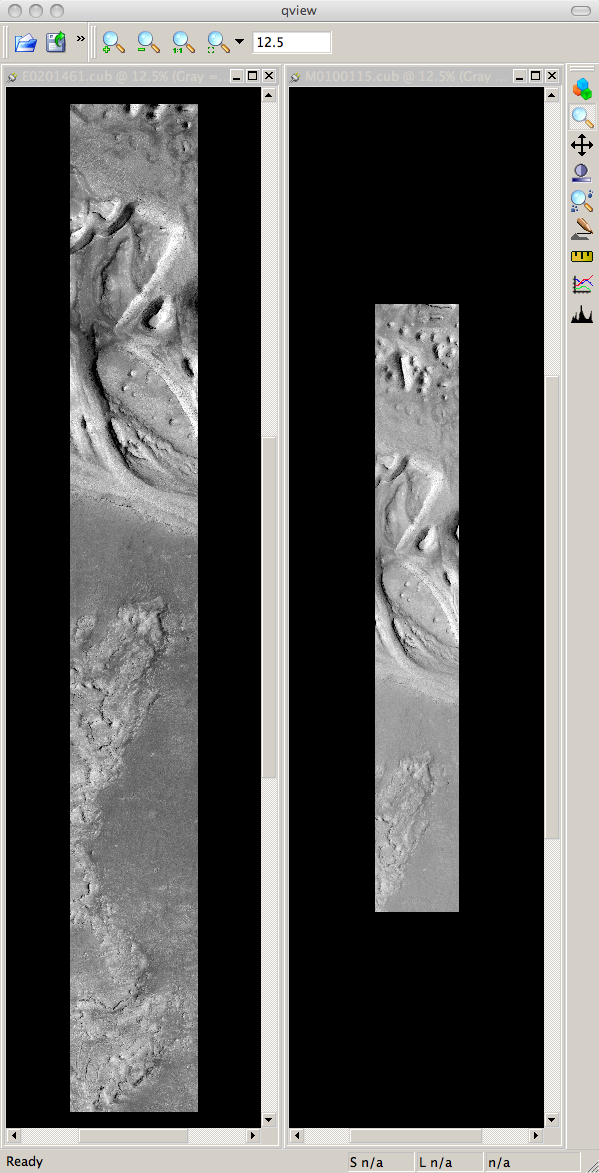
\includegraphics[height=3.7in]{images/p19-images.png}
\hfill
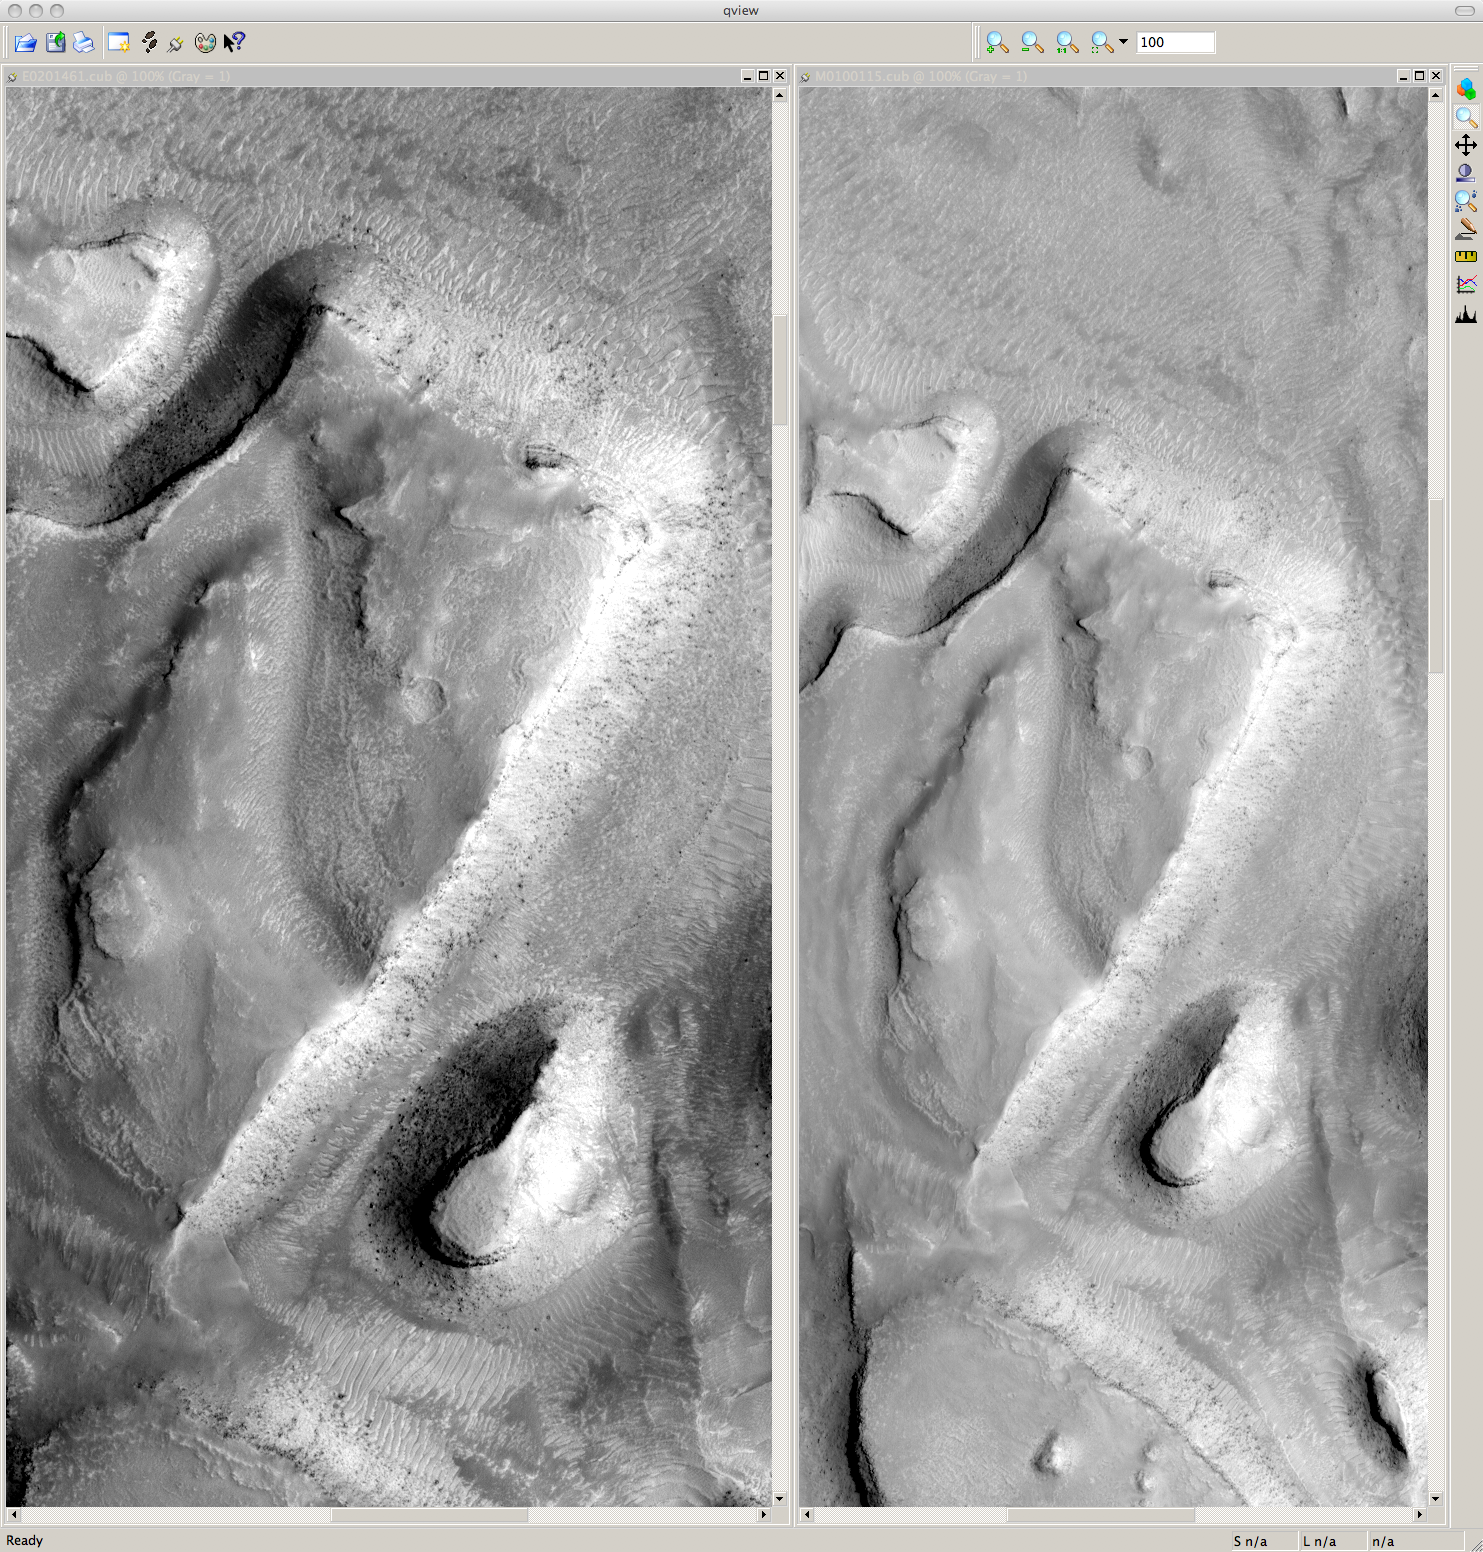
\includegraphics[height=3.7in]{images/p19-images_zoom.png}
\end{minipage}
\hfill
\begin{minipage}{1.3in}
\caption[P19 images open in qview zoomed in]{
    \label{p19-images}
    This figure shows \texttt{E0201461.cub} and \texttt{M0100115.cub}
    open in ISIS's qview program.  The view on the left shows their
    full extents at the same zoom level, showing how they have
    different ground scales.  The view on the right shows both images
    zoomed in on the same feature.  }
\end{minipage}
\end{figure}

\subsection{Map Projecting Images}

The images also need to be rectified (or aligned).  There are many
ways to do this (including using \texttt{DO\_INTERESTPOINT\_ALIGNMENT}
in \texttt{stereo}'s \texttt{stereo.default} file).  The most
straightforward process is to align the images by map projecting
them in \ac{ISIS}. This example continues with the files from above,
\texttt{E0201461.cub} and \texttt{M010015.cub}.

The \ac{ISIS} \texttt{cam2map} program will map-project these images:

\begin{verbatim}
  ISIS 3> cam2map from=M0100115.cub to=M0100115.map.cub
  ISIS 3> cam2map from=E0201461.cub to=E0201461.map.cub map=M0100115.map.cub matchmap=true
\end{verbatim}

Notice the order in which the images were run through
\texttt{cam2map}.  The first projection with \texttt{M0100115.cub}
produced a map-projected image centered on the center of that image.
The projection of \texttt{E0201461.cub} used the \texttt{map=}
parameter to indicate that \texttt{cam2map} should use the same map
projection parameters as those of \texttt{M0100115.map.cub} (including
center of projection, map extents, map scale, etc.) in creating the
projected image.  By map projecting the image with the worse
resolution first, and then matching to that, we ensure two things: (1)
that the second image is summed or scaled down instead of being
magnified up, and (2) that we are minimizing the file sizes to make
processing in the Stereo Pipeline more efficient.

Technically, the same end result could be achieved by using the
\texttt{mocproc} program alone, and using its \texttt{map=} option (it
behaves identically to \texttt{cam2map}), but this would not allow you
to force the two images into the same map projection.  Furthermore, if
you choose to conduct bundle adjustment (see Chapter
\ref{ch:bundle_adjustment}, page \pageref{ch:bundle_adjustment}) as a
pre-processing step, you would do so between \texttt{mocproc} and
\texttt{cam2map}.

The above procedure is in the case of two images which cover similar
real estate on the ground.  If you have a pair of images where one
image has a footprint on the ground that is much larger than the
other, only the area that is common to both (the mathematical
intersection of their areas) should be kept to perform correlation
on (since non-overlapping regions don't contribute to the stereo
solution).  If the image with the larger footprint size also happens
to be the image with the better resolution (i.e. the image run through
\texttt{cam2map} second with the \texttt{map=} parameter), then the
above \texttt{cam2map} procedure with \texttt{matchmap=true} will take care
of it just fine.  Otherwise you'll need to figure out the latitude
and longitude boundaries of the intersection boundary 
(with the \ac{ISIS} \texttt{camrange} program).  Then use that smaller
boundary as the arguments to the \texttt{MINLAT}, \texttt{MAXLAT},
\texttt{MINLON}, and \texttt{MAXLON} parameters of the first run
of \texttt{cam2map}.  So in the above example, after \texttt{mocproc} with
\texttt{Mapping= NO} you'd do this:

\begin{Verbatim}[commandchars=\\\{\}]
  ISIS 3> camrange fr= M0100115.cub
          \textnormal{[ ... lots of} camrange \textnormal{ output omitted ... ]}
  Group = UniversalGroundRange
    LatitudeType       = Planetocentric
    LongitudeDirection = PositiveEast
    LongitudeDomain    = 360
    MinimumLatitude    = 34.079818835324
    MaximumLatitude    = 34.436797628116
    MinimumLongitude   = 141.50666207418
    MaximumLongitude   = 141.62534719278
  End_Group
          \textnormal{[ ... more output of} camrange \textnormal{ omitted ... ]}

  ISIS 3> camrange fr= E0201461.cub
          \textnormal{[ ... lots of} camrange \textnormal{ output omitted ... ]}
  Group = UniversalGroundRange
    LatitudeType       = Planetocentric
    LongitudeDirection = PositiveEast
    LongitudeDomain    = 360
    MinimumLatitude    = 34.103893080982
    MaximumLatitude    = 34.547719435156
    MinimumLongitude   = 141.48853937384
    MaximumLongitude   = 141.62919740048
  End_Group
          \textnormal{[ ... more output of} camrange \textnormal{ omitted ... ]}
\end{Verbatim}

Now compare the boundaries of the two above and determine the intersection to use as the boundaries for \texttt{cam2map}:

\begin{Verbatim}
  ISIS 3> cam2map from=M0100115.cub to=M0100115.map.cub MINLAT= 34.10 MAXLAT= 34.44 \
                  MINLON= 141.50 MAXLON= 141.63
  ISIS 3> cam2map from=E0201461.cub to=E0201461.map.cub map=M0100115.map.cub matchmap=true
\end{Verbatim}

You only have to do the boundaries explicitly for the first run of
\texttt{cam2map}, because the second one uses the \texttt{map=}
parameter to mimic the map projection of the first.  These two
images aren't radically different in areal coverage, so this isn't
really necessary for these images, its just an example.

\vfill

\section{Running the Stereo Pipeline}

Once the data has been prepared for processing, we envoke the the
\texttt{stereo} program (page \pageref{stereo}).  The \texttt{stereo}
program can generate a number of output files, and you may find it
helpful to create a directory to store the results of stereo
processing, as illustrated below.

\begin{verbatim}
    ISIS 3> ls
    E0201461.cub   E0201461.map.cub   M0100115.cub   M0100115.map.cub
    ISIS 3> mkdir results
\end{verbatim}
\noindent

\subsection{Setting Options in the \texttt{stereo.default} File}

The \texttt{stereo} program requires a \texttt{stereo.default} file
that contains settings that effect the stereo reconstruction process.
Its contents can be altered for your needs; details are found in
appendix \ref{ch:stereodefault} on page \pageref{ch:stereodefault}.
You may find it useful to save multiple versions of the
\texttt{stereo.default} file for various processing needs. If you do
this, be sure to specify a configuration file by invoking
\texttt{stereo} with the \texttt{-s} option.  If this option is not
given, the \texttt{stereo} program will search for a file named
\texttt{stereo.default} in the current working directory.

There is a \texttt{stereo.default} file included with the example data
set that is different from the example \texttt{stereo.default.example}
file distributed with the Stereo Pipeline.  The
\texttt{stereo.default} included with the example data has a smaller
correlation window (smaller values for the \texttt{H\_CORR\_*} and
\texttt{V\_CORR\_*} variables) that is more suited to the MOC data.

Alternatively, it is possible to not have to define the
\texttt{H\_CORR\_*} and \texttt{V\_CORR\_*} in
\texttt{stereo.default}. If no such options are specified,
\texttt{stereo} will attempt to guess the correct search range. The
guess is printed along with the rest of the program output.  If this
technique does not produce satisfactory results, then it can at least
be used as a starting point for picking a better search range by hand.

For this example use the \texttt{stereo.default} that is included with
the example data set. It has these key properties:

\begin{verbatim}
        DO_INTERESTPOINT_ALIGNMENT 0
        H_CORR_MIN -35
        H_CORR_MAX -15
        V_CORR_MIN -280
        V_CORR_MAX -265
\end{verbatim}
\noindent

The first says, \emph{`Don't do interest point alignment!'} since we
have map-projected the images. The other four lines define the range
that should be searched by scanning a template from the left image
over the right image. The values above are tuned to the range of
offsets that is found in this particular set of map projected images.

Given that we map projected the images using the same settings, you
may be wondering why would there still be an offset. The reason is
twofold: (1) the camera position may be slightly off, resulting in
slight mis-alignment between stereo images; or (2) \ac{ISIS} doesn't
have a perfect surface to project onto during map projection, so small
terrain features still produce changes in perspective.  (In fact,
these are precisely the features we are hoping to detect!)

\begin{center}
\fcolorbox{black}{lgray}{ \begin{minipage}{5.5in}

   Given the uncertainties due to (1) and (2) above, it can be tricky
   to select a good search range for the \texttt{stereo.default} file.
   One way is to let \texttt{stereo} perform one round of auto search
   range search.  Look at the results using the
   \texttt{disparitydebug} program.  The output images will clearly
   show good data or bad data depending on whether the search range is
   correct.  If the edges of these images look degrade, then the
   search range may need to be expanded by hand.

   The worst case scenario is to determine search range by hand by
   opening both images in qview and comparing the coordinates of
   points that you can match visually. Subtract locations from the
   first image from the second image, will yield offsets that must be
   in the search range.  Build a bounding box around several of these
   sampled offset,s and then expand the box by 50\%.  This will
   produce good results in most images. Future versions of the
   software will try to better assist the user in automatically
   determining the correlation window.

\end{minipage}}
\end{center}

\subsection{Performing Stereo Correlation}

Here is how the \texttt{stereo} program is invoked:

\begin{verbatim}
    ISIS 3> stereo E0201461.map.cub M0100115.map.cub results/E0201461-M0100115
\end{verbatim}

\noindent
That last option (\texttt{results/E0201461-M0100115}) is a prefix that
is used when generating names for \texttt{stereo} output files.  In
this case the first part is \texttt{results/}, which causes the
program to generate results in that directory with filename that start
with \texttt{E0201461-M0100115}. If instead that last text was
\texttt{E0201461-M0100115} it would have created a collection of files
that start with \texttt{E0201461-M0100115} in the {\em same} directory as
the input files.

\subsection{Diagnosing Problems}

Once invoked, \texttt{stereo} proceeds through several stages that are
detailed on page \pageref{entrypoints}.  Intermediate and final output
files are generated as it goes.  See Appendix
\ref{chapter:outputfiles}, page \pageref{chapter:outputfiles} for a
comprehensive listing.  Many of these files are useful diagnosing and
debugging problems.  For example, as Figure~\ref{p19-stereo-output}
shows, a quick look at some of the TIFF files in the \texttt{results/}
directory provides some insight into the process.

\begin{figure}
\begin{center}
\includegraphics[width=5in]{images/p19-stereo-output.png}
\caption[P19 stereo output images]{
    \label{p19-stereo-output}
	These are the four viewable \texttt{.tif} files created by the
        \texttt{stereo} program.  On the left are the two aligned,
        pre-processed images: (\texttt{E0201461-M0100115-L.tif} and
        \texttt{E0201461-M0100115-R.tif}).  The two are mask images
        (\texttt{E0201461-M0100115-lMask.tif} and
        \texttt{E0201461-M0100115-rMask.tif}), which indicate which
        pixels in the aligned images are good to use in stereo
        correlation.  The image on the right is the ``Good Pixel
        map'', (\texttt{E0201461-M0100115-GoodPixelMap.tif}), which
        indicates (in gray) which were successfully matched with the
        correlator, and (in red) those that were not matched.}
\end{center}
\end{figure}

% \begin{figure}
% \begin{center}
% 
\includegraphics[height=8in]{images/p19-goodpixel.png}
% \caption[P19 good pixel image]{
%     \label{p19-goodpixel}
% 	The Good Pixel map.
% 	Red pixels are not useful for alignment.
%     }
% \end{center}
% \end{figure}
%
% \begin{figure}
% \begin{center}
% 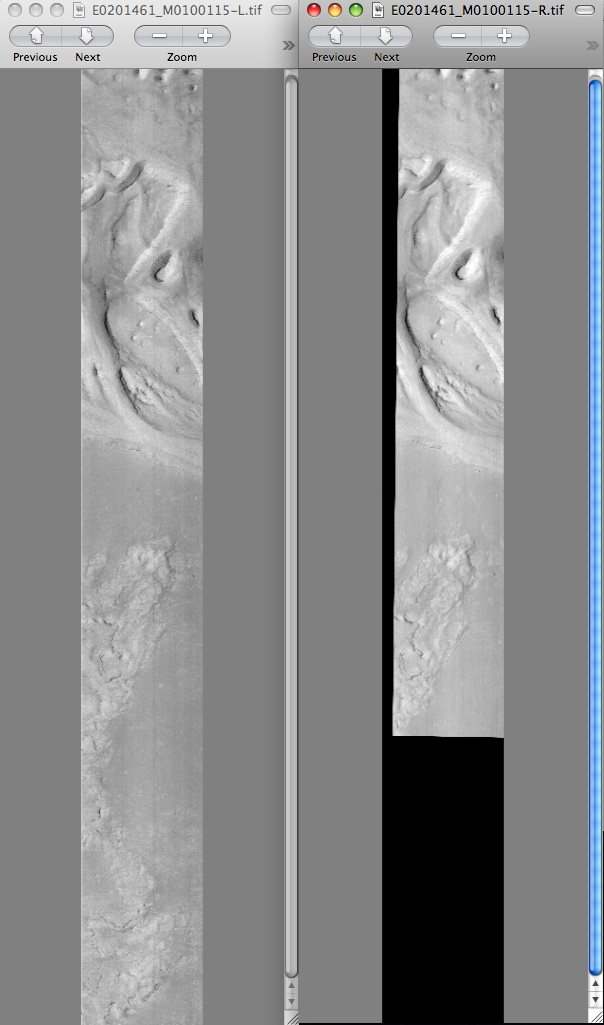
\includegraphics[width=3in]{images/p19-aligned.png}
% \caption[P19 aligned image]{
%     \label{p19-aligned}
% 	The left and right aligned images.
%     }
% \end{center}
% \end{figure}

Perhaps the most important file for assessing the quality of your
results is the good pixel image,
\\ (\texttt{E0201461-M0100115-GoodPixelMap.tif}).  If this file shows
mostly good, gray pixels in the overlap area (the area that is white
in both the \texttt{E0201461-M0100115-lMask.tif} and
\texttt{E0201461-M0100115-rMask.tif} files), then your results are
just fine.  If the good pixel image shows missing data, signified by
red pixels in the overlap area, then you need to go back and tune your
\texttt{stereo.default} file until your results improve.  This might
be a good time to make a copy of \texttt{stereo.default} as you tune
the parameters to improve the results.

Another handy debugging tool is the \texttt{disparitydebug} program,
which allows you to generate viewable versions of the intermediate
results from the stereo correlation algorithm.
\texttt{disparitydebug} converts information in \texttt{.exr}
disparity files into two TIFF images that contain horizontal and
vertical components of the disparity (i.e. matching offsets for each
pixel in the horizontal and vertical directions).  There are actually
four flavors of disparity map: the \texttt{-D.exr}, the
\texttt{-R.exr}, the \texttt{-F-corrected.exr}, and \texttt{-F.exr}.
You can run \texttt{disparitydebug} on any of them.  Each shows the
disparity map at the different stages of processing.

\begin{verbatim}
    ISIS 3> cd results
    ISIS 3> disparitydebug E0201461-M0100115-F.exr
\end{verbatim}

If the TIFF files from \texttt{disparitydebug} look okay, then the
point cloud image are most likely ready for post-processing.  You can
proceed to make a mesh or a \ac{DEM} by processing
\texttt{E0201461-M0100115-PC.tif} using the \texttt{point2mesh} or
\texttt{point2dem} tools, respectively.

\begin{figure}[t!]
\begin{minipage}{4in}
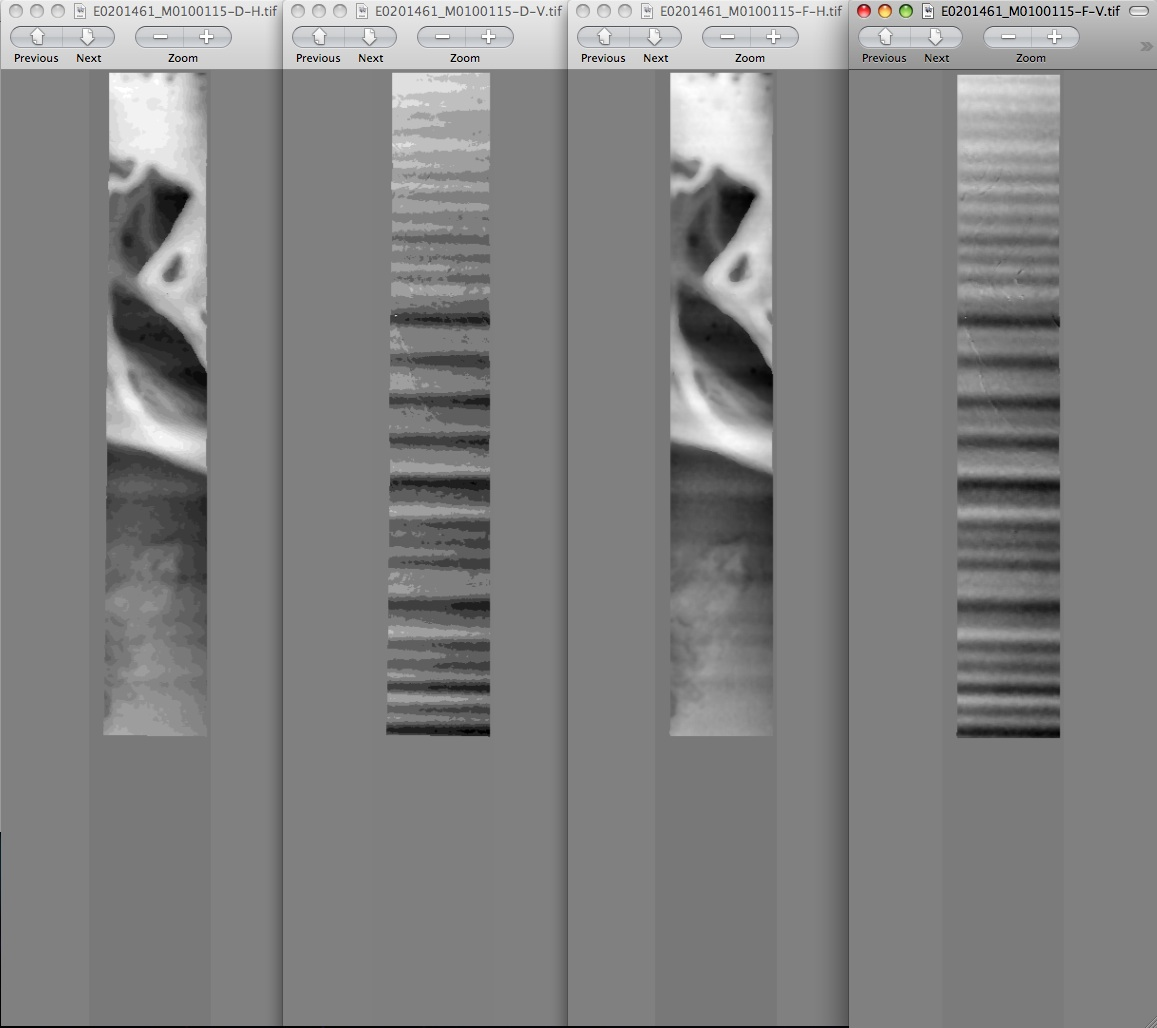
\includegraphics[width=4in]{images/p19-disparity.png}
\end{minipage}
\hfill
\begin{minipage}{2.7in}
\caption[P19 disparity images]{
    \label{p19-disparity}
	Disparity images produced using the \texttt{disparitydebug}
        tool.  The two images on the left are the
        \texttt{E0201461-M0100115-D-H.tif} and
        \texttt{E0201461-M0100115-D-V.tif} files, which are the raw
        horizontal and vertical disparity components produced by the
        disparity map initialization phase.  The two images on the
        right are \texttt{E0201461-M0100115-F-H.tif} and
        \texttt{E0201461-M0100115-F-V.tif}, which are the final
        filtered, sub-pixel-refined disparity maps that a fed into the
        Triangulation phase to build the point cloud image.  Since
        these MOC images were acquired by rolling the spacecraft
        across-track, most of the disparity that represents topography
        is present in the horizontal disparity map.  The vertical
        disparity map shows disparity due to ``washboarding,'' which
        is not from topography but from spacecraft movement. Note
        however that the horizontal and vertical disparity images are
        normalized independently.  Although both have the same range
        of gray values from white to black, they represent
        significantly different absolute ranges of disparity.}
\end{minipage}
\end{figure}

\section{Visualizing the Results}

When \texttt{stereo} finishes, it will have produced a point cloud
image.  At this point, many kinds of data products can be built from
the \texttt{E0201461-M0100115-PC.tif} point cloud file.

\subsection{Building a 3D Model}

If you wish to see the data in an interactive 3D browser, then you can
generate a 3D object file using the \texttt{point2mesh} command (page
\pageref{point2mesh}). The resulting file is stored in Open Scene
Graph binary format \cite{OSG_website}.  It can be viewed with
\texttt{osgviewer} (the Open Scene Graph Viewer program, distributed
with the binary version of the Stereo Pipeline).  The
\texttt{point2mesh} program takes the point cloud file and the left
normalized image as inputs:

\begin{verbatim}
    ISIS 3> point2mesh E0201461-M0100115-PC.tif E0201461-M0100115-L.tif -l
\end{verbatim}

\noindent
When the \texttt{osgviewer} program starts, you may want to toggle the
lighting with the `L' key, toggle texturing with the 'T' key, and
toggle wireframe mode with the 'W'.  Press '?' to see a variety of
other interactive options.

\begin{figure}[t]
\begin{minipage}{5in}
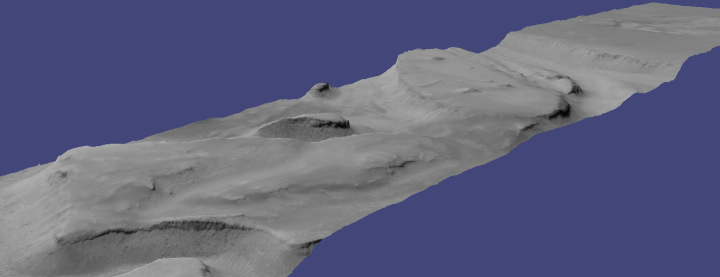
\includegraphics[width=5in]{images/p19-osg.png}
\end{minipage}
\hfill
\begin{minipage}{1.7in}
\caption[P19 in OSG]{
    \label{p19-osg}
	The \texttt{E0201461-M0100115.ive} file displayed in the OSG
        Viewer.  }
\end{minipage}
\end{figure}

\subsection{Building a Digital Elevation Model}

The \texttt{point2dem} program (page \pageref{point2dem}) creates a
\ac{DEM} from the point cloud file.

\begin{verbatim}
    ISIS 3> point2dem --xyz-to-lonlat E0201461-M0100115-PC.tif
\end{verbatim}

\noindent
The resulting TIFF file is map projected and will contain
georeferencing information stored as GeoTIFF tags.  The
``--xyz-to-lonlat'' option is {\em required} in most common uses, as
it transforms the results from a cartesion, body-centered coordinate
system to the longitude, latitude, altitude spherical coordinate
system.  You can specify a coordinate system (e.g., mercator,
sinusoidal) and a reference spheroid (i.e., calculated for the Moon or
Mars).

\begin{verbatim}
    ISIS 3> point2dem --xyz-to-lonlat -r mars E0201461-M0100115-PC.tif
\end{verbatim}

\noindent
This product is suitable for scientific use, and can be imported into
a variety of GIS platforms.  However, the resulting file,
\texttt{E0201461-M0100115-DEM.tif}, will have 32-bit floating point
pixels, and will not render well in typical image viewers.

The \texttt{point2dem} program can also be used to orthoproject raw
satellite imagery onto the \ac{DEM}. To do this, invoke
\texttt{point2dem} just as before, but add the \texttt{--orthoimage}
option and specify the use of the left image file as the texture file
to use for the projection:

\begin{verbatim}
    ISIS 3> point2dem --xyz-to-lonlat -r mars --orthoimage E0201461-M0100115-L.tif \
        E0201461-M0100115-PC.tif
\end{verbatim}

\noindent
The \texttt{point2dem} program can be used in many different ways.  Be
sure to explore all of the options.

\begin{figure}
\begin{minipage}{5in}
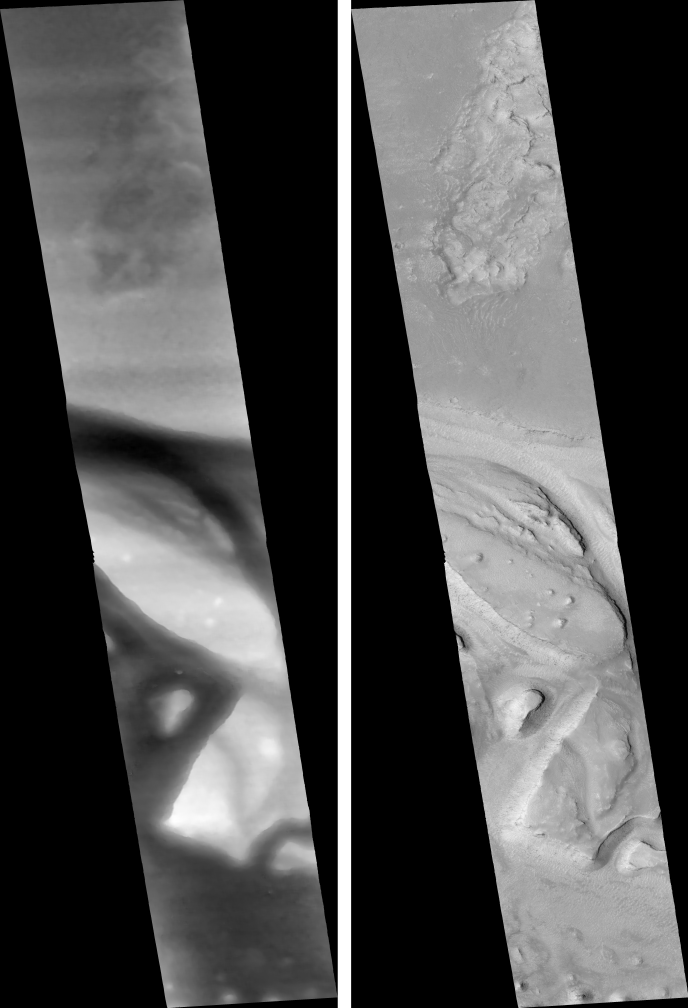
\includegraphics[width=5in]{images/p19-norm_ortho.png}
\end{minipage}
\hfill
\begin{minipage}{1.5in}
\caption[P19 Normalized DEM and Orthophoto]{
    \label{p19-norm_ortho}
	The image on the left is a normalized DEM (generated using the
        \texttt{-n} option), which shows low terrain values as black
        and high terrain values as white.  The image on the right is
        the left input image projected onto the DEM (created using the
        \texttt{--orthoimage} option to \texttt{point2dem}).  }
\end{minipage} \end{figure}

% \begin{figure}
% \begin{center}
% 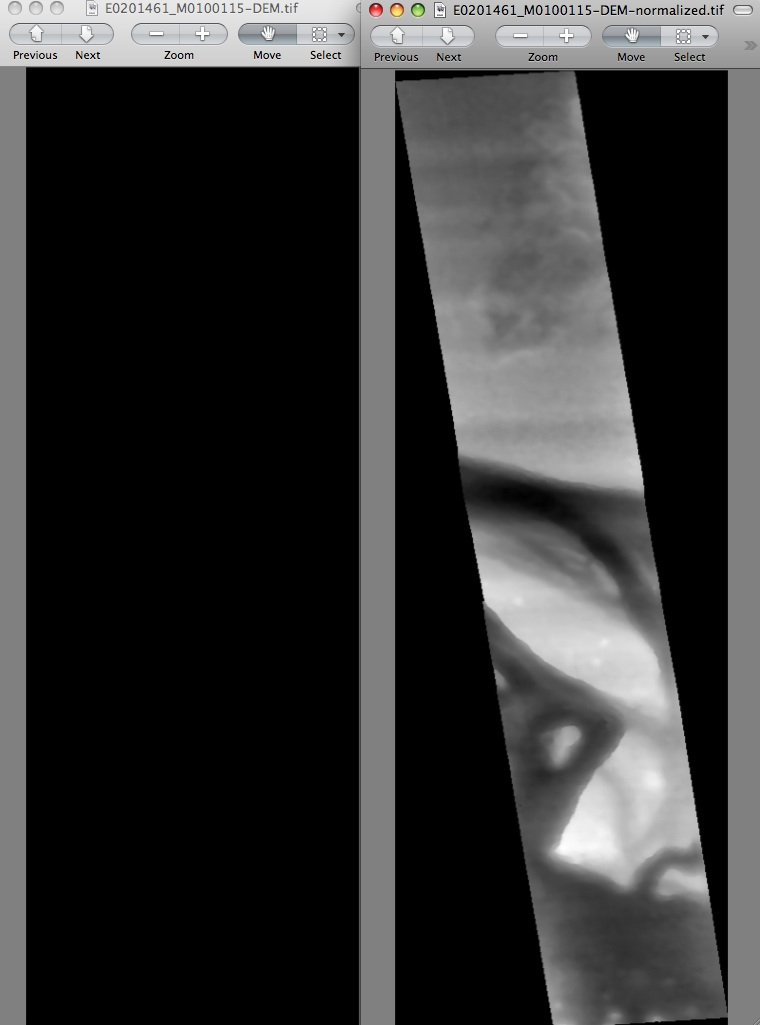
\includegraphics[width=4in]{images/p19-dems.png}
% \caption[P19 dem images]{
%     \label{p19-dems}
% 	The non-normalized and normalized DEMs. Note that the
% 	non-normalized version contains floating point pixel values
% 	and will not open in most image viewing programs which
% 	expect integer pixel values between 0 and 255 (which is
% 	what the normalized version does for you).
%     }
% \end{center}
% \end{figure}
%
% \begin{figure}
% \begin{center}
% \includegraphics[width=3in]{images/p19-ortho.png}
% \caption[P19 orthophoto]{
%     \label{p19-ortho}
% 	The left image orthoprojected onto the DEM.
%     }
% \end{center}
% \end{figure}

\subsection{Generating Color Hillshade Maps}

Once you have generated a \ac{DEM} file, you can use the Vision Workbench's
\texttt{colormap} and \texttt{hillshade} tools to create colorized
and/or shaded relief images.

To create a colorized version of the \ac{DEM}, you need only specify
the \ac{DEM} file to use. The colormap is applied to the full range of
the DEM, which is computed automatically.  Alternatively you can
specific your own min and max range for the color map.

\begin{verbatim}
    ISIS 3> colormap E0201461-M0100115-DEM.tif -o hrad-colorized.tif
\end{verbatim}

To create a hillshade of the \ac{DEM}, specify the \ac{DEM} file to
use. You can control the azimuth and elevation of the light source
using the \texttt{-a} and \texttt{-e} options.

\begin{verbatim}
    ISIS 3> hillshade E0201461-M0100115-DEM.tif -o hrad-shaded.tif -e 25
\end{verbatim}

To create a colorized version of the shaded relief file, specify
the \ac{DEM} and the shaded relief file that should be used:

\begin{verbatim}
    ISIS 3> colormap E0201461-M0100115-DEM.tif -s hrad-shaded.tif -o hrad-color-shaded.tif
\end{verbatim}

\begin{figure}
\begin{center}
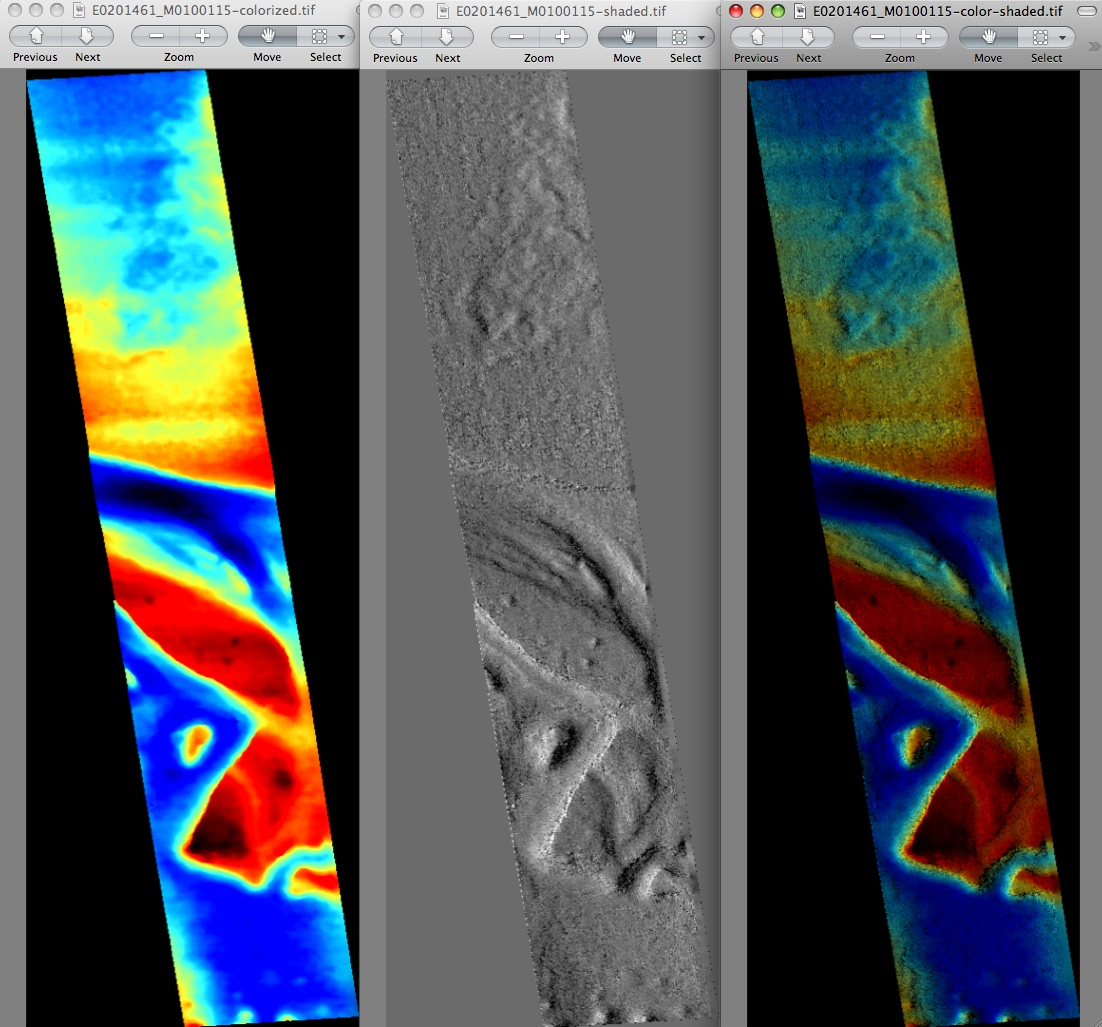
\includegraphics[width=5in]{images/p19-colorized-shaded.png}
\caption[Hrad colorized and shaded relief]{
    \label{hrad-color}
	The colorized DEM, the shaded relief image, and the colorized hillshade.
    }
\end{center}
\end{figure}

\subsection{Building Overlays for Moon and Mars mode in Google Earth}

The final program in the Stereo Pipeline package that this tutorial
will address is \texttt{image2qtree}.  This tool was designed to
create tiled, multi-resolution overlays for Google Earth.  In addition
to generating image tiles, it produces a metadata tree in KML format
that can be loaded from your local hard drive or streamed from a
remote server over the Internet.  

The \texttt{image2qtree} program can only be used on 8-bit image files
with georeferencing information (e.g. grayscale or RGB geotiff
images). In this example, it can be used to process
\texttt{E0201461-M0100115-DEM-normalized.tif},
\texttt{E0201461-M0100115-DRG.tif} \texttt{hrad-shaded.tif},
\texttt{hrad-colorized.tif}, and \texttt{hrad-shaded-colorized.tif}

\begin{verbatim}
    ISIS 3> image2qtree hrad-shaded-colorized.tif -m kml --draw-order 100
\end{verbatim}

\begin{figure}[b!]
\begin{center}
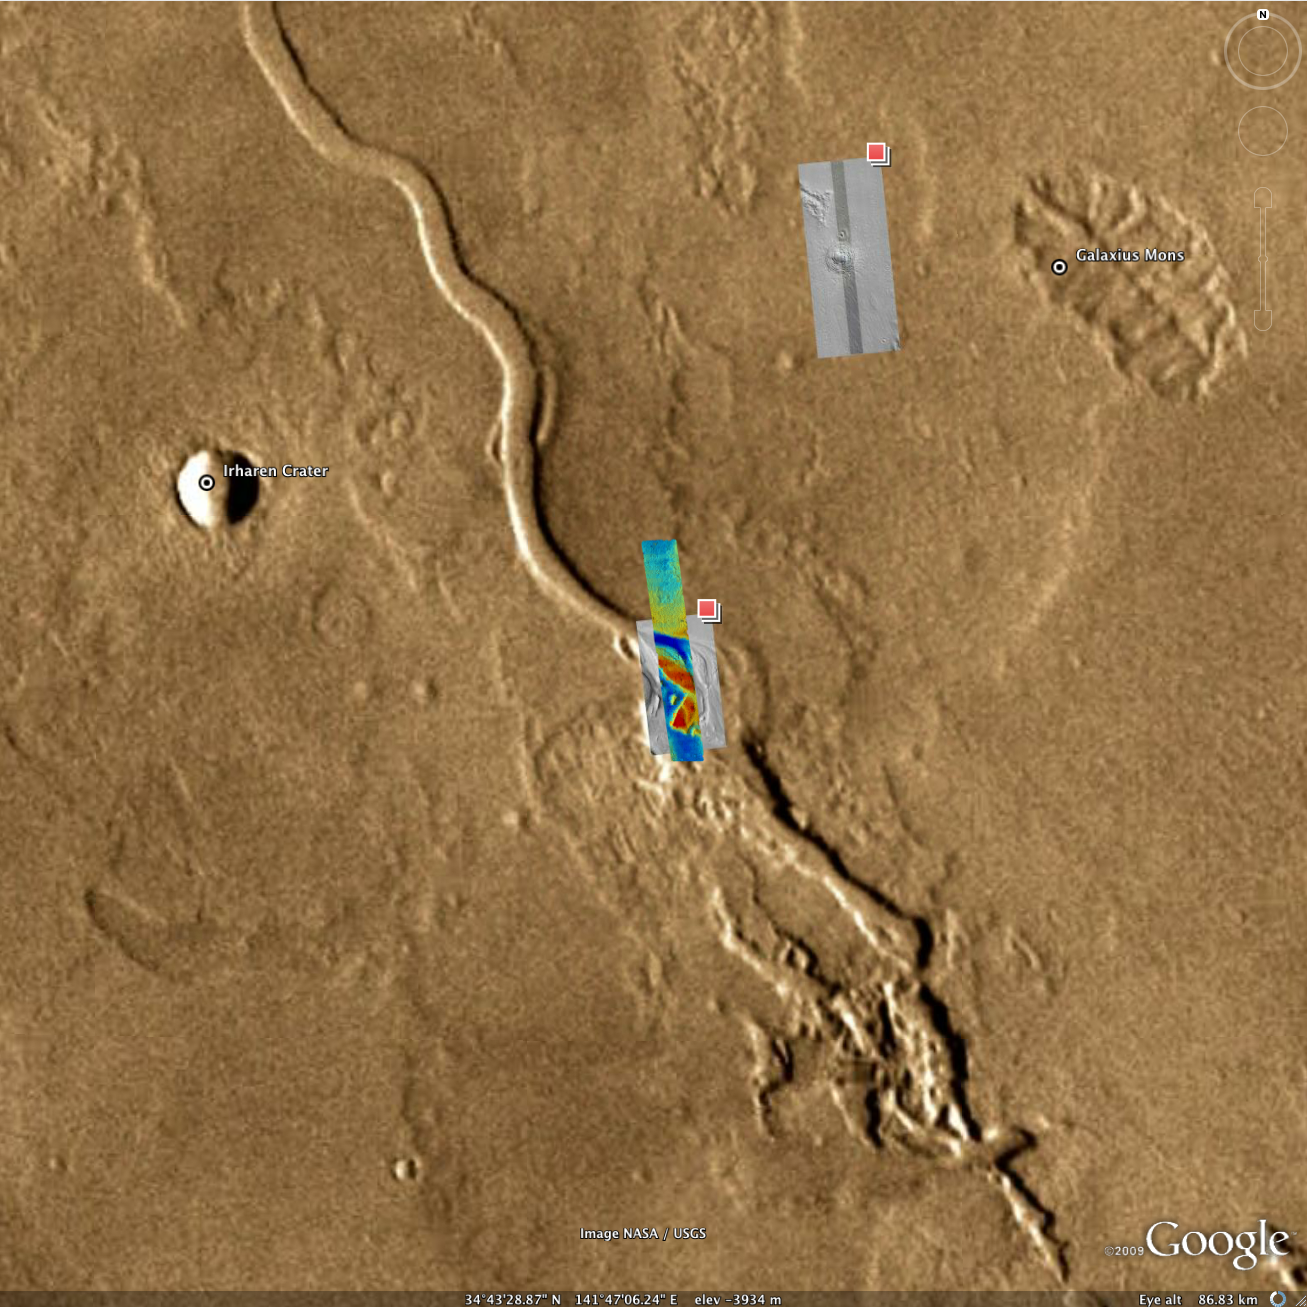
\includegraphics[width=6in]{images/p19-googlemars.png}
\caption[Hrad shaded colorized DEM as a KML overlay] {
    \label{hrad-kml}
        The colorized hillshade DEM as a KML overlay.  }
\end{center}
\end{figure}
